\documentclass[../machine_learning_scikit.tex]{subfiles}

\begin{document}

    \chapter{Module 1}

    The goal of this chapter is to explore the foundational concepts of machine learning, focusing on how algorithms can transform data into knowledge. We delve into the practical applications of supervised and unsupervised learning, equipping you with the skills to implement these techniques using Python tools for effective data analysis and prediction.
    
    \begin{obs}[\textbf{Learning Objectives}]
        \textbf{Learning Objectives}:
        \begin{itemize}
            \item Analyze data patterns to make future predictions.
            \item Design systems for supervised and unsupervised learning.
            \item Implement machine learning algorithms using Python tools.
        \end{itemize}
    \end{obs}
        
    \section{Overview}

    The goal basically is to learn machine learning using Python libraries such as Scikit-Learn and PyTorch.

    \section{Giving computers the ability to learn from data}

    So, basically in this scenario we will do the following:
    \begin{itemize}
        \item Implement machine learning algorithms using Python tools.
        \item Desing systems for supervised and unsupervised learning.
        \item Analyze data patterns to make future predictions.
    \end{itemize}

    \section{Introduction}

    \begin{mydef}[\textbf{Machine Learning}]
        \textbf{Machine learning} is the\textit{ application and science of algorithms that make sense of data}.
    \end{mydef}

    The goal of this section is to introduce some of the main concepts and different types of machine learning, together with a basic introduction to the relevant terminology. The goal is to stablish the groundwork for successfully using machine learning techniques for practical prolem solving.

    \subsection{The Three Different Types of Machine Learning}

    In this age, we have a large amount of structured and non-structured data.

    \begin{mydef}[\textbf{Structured and Non-structured Data}]
        \textbf{Structured data} refers \textit{to information that is organized in a predefined format}, typically within a fixed schema, such as rows and columns in a database or spreadsheet

        In contrast, \textbf{non-structured data} \textit{lacks a predefined format or structure and exists in its native, raw state}. It is typically qualitative and encompasses a wide variety of formats such as text documents, emails, social media posts, images, videos, and audio files.
    \end{mydef}

    One of the main goals of machine learning is to extract knowledge from data in order to make predictions.

    \begin{obs}[\textbf{Use of Machine Learning}]
        \textbf{Machine Learning} \textit{offers a more efficient alternative for capturing the knowledge in data to improve the performance of predictive models and make data-driven decisions}.
    \end{obs}
    
    \begin{idea}[\textbf{Note on the use of Machine Learning and some of its Applications}]
        Also, notable progress has been made in medical applications; for example, researchers demonstrated that deep learning models can detect skin cancer with near-human accuracy \href{https://www.nature.com/articles/nature21056}{link to article}.
        
        Another milestone was recently achieved by researchers at DeepMind, who used deep learning to predict 3D protein structures, outperforming physics-based approaches by a substantial margin \href{https://deepmind.com/blog/article/alphafold-a-solution-to-a-50-year-old-grand-challenge-in-biology}{link to article}.  
    \end{idea}
    
    There are three types of machine learning: \textbf{supervised learning}, \textbf{unsupervised learning}, and \textbf{reinforcement learning}. There are fundamental differences between these three types of machine learning and we will look at each of them in detail with some notes on its possible applications.
 
    \begin{longtable}{l p{7cm}}
        \toprule
        \multicolumn{2}{c}{\textbf{Three Types of Machine Learning}} \\
        \midrule
        \endfirsthead
        
        \toprule
        \multicolumn{2}{c}{\textbf{Three Types of Machine Learning}} \\
        \midrule
        \endhead
        
        \bottomrule
        \caption{Three Types of Machine Learning.}
        \label{table:types_machine_learning}
        \endlastfoot
        
        \multirow{3}{*}{Supervised learning} 
        & • Labeled data \\
        & • Direct feedback \\
        & • Predict outcome/future \\
        \hline
        \multirow{3}{*}{Unsupervised learning}
        & • No labels/targets \\
        & • No feedback \\
        & • Find hidden structure in data \\
        \hline
        \multirow{3}{*}{Reinforcement learning}
        & • Decision process \\
        & • Reward system \\
        & • Learn series of actions \\
    \end{longtable}

    \subsection{Supervised Learning}

    The main goal of \textbf{supervised learning} is to \textit{learn a model from labeled training data that allows us to make predicitons about unseen or future data}.

    The term \textit{supervised} refers to a set of training examples (data inputs), where the desired output signals (labels) are already known.

    \begin{mydef}[\textbf{Supervised Learning}]
        \textbf{Supervised learning} is the \textit{process of modeling the relationship between data inputs and the labels}.
    \end{mydef}

    We can think of supervised learning as \textit{label learning}.

    \begin{figure}[h]
        \begin{minipage}{\textwidth}
            \centering
            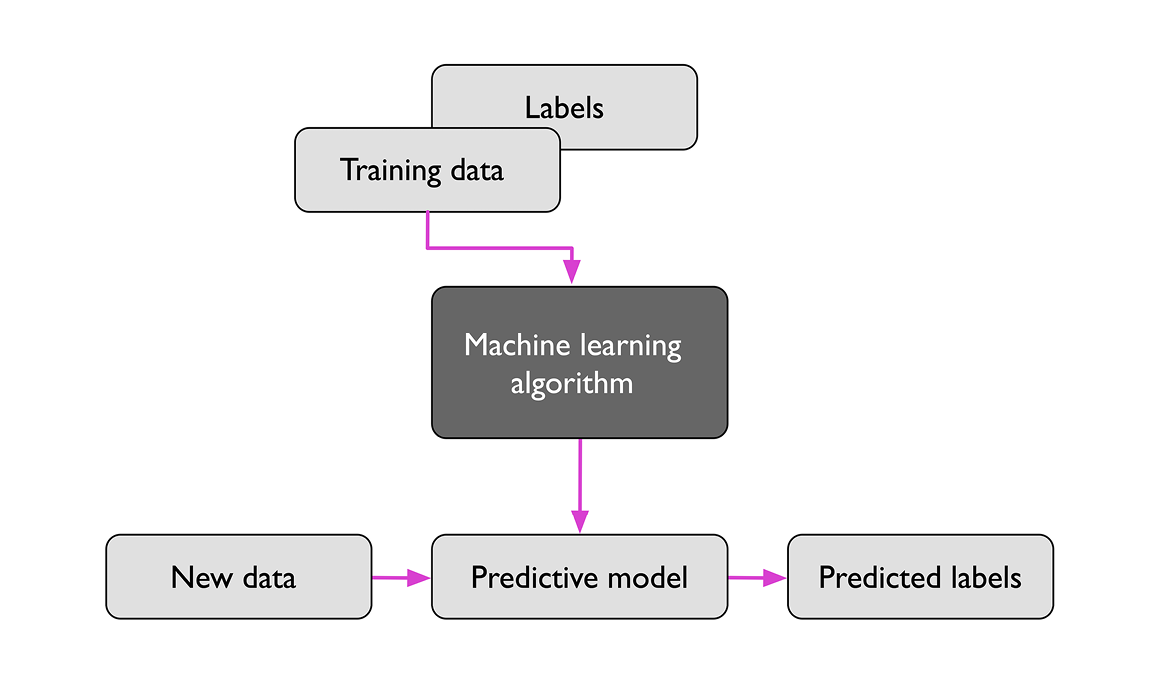
\includegraphics[scale=1]{images/supervised_learning_process.png} \\
            \caption{General Process of Supervised Learning}
            \label{figure:general_process_supervised_learning}
        \end{minipage}
    \end{figure}

    \begin{exa}[\textbf{Example of Supervised Learning}]
        Lets consider the example of email spam filtering. We can train a model using a supervised machine learning algorithm on a corpus of labeled emails, which are correctly marked as spam or non-spam.

        To predict whether a new email belongs to either of the two categories, a supervised learning task with discrete class labels, such as in the previous email spam filtering example.
        
        This is called a \textbf{classification task}. Another subcategory of supervised learning is \textbf{regression}, where the outcome signal is a continous value.
    \end{exa}

    \subsection{Classification for Predicting Class Labels}

    \begin{mydef}[\textbf{Classification}]
        \textbf{Classification} is \textit{a subcategory of supervised learning, where the goal is to predict the categorical class labels of new instances or data points based on past observations}.
    \end{mydef}

    Thos class labels are discrete, unordered values that can be understood as the group memberships of the data points. The previously mentioned example of email spam detection represents a typical example of a binary classification task, where the machine learning algorithm learns a set of rules to distinguish between two possible classes: spam and no-spam emails.

    \begin{figure}[h]
        \begin{minipage}{\textwidth}
            \centering
            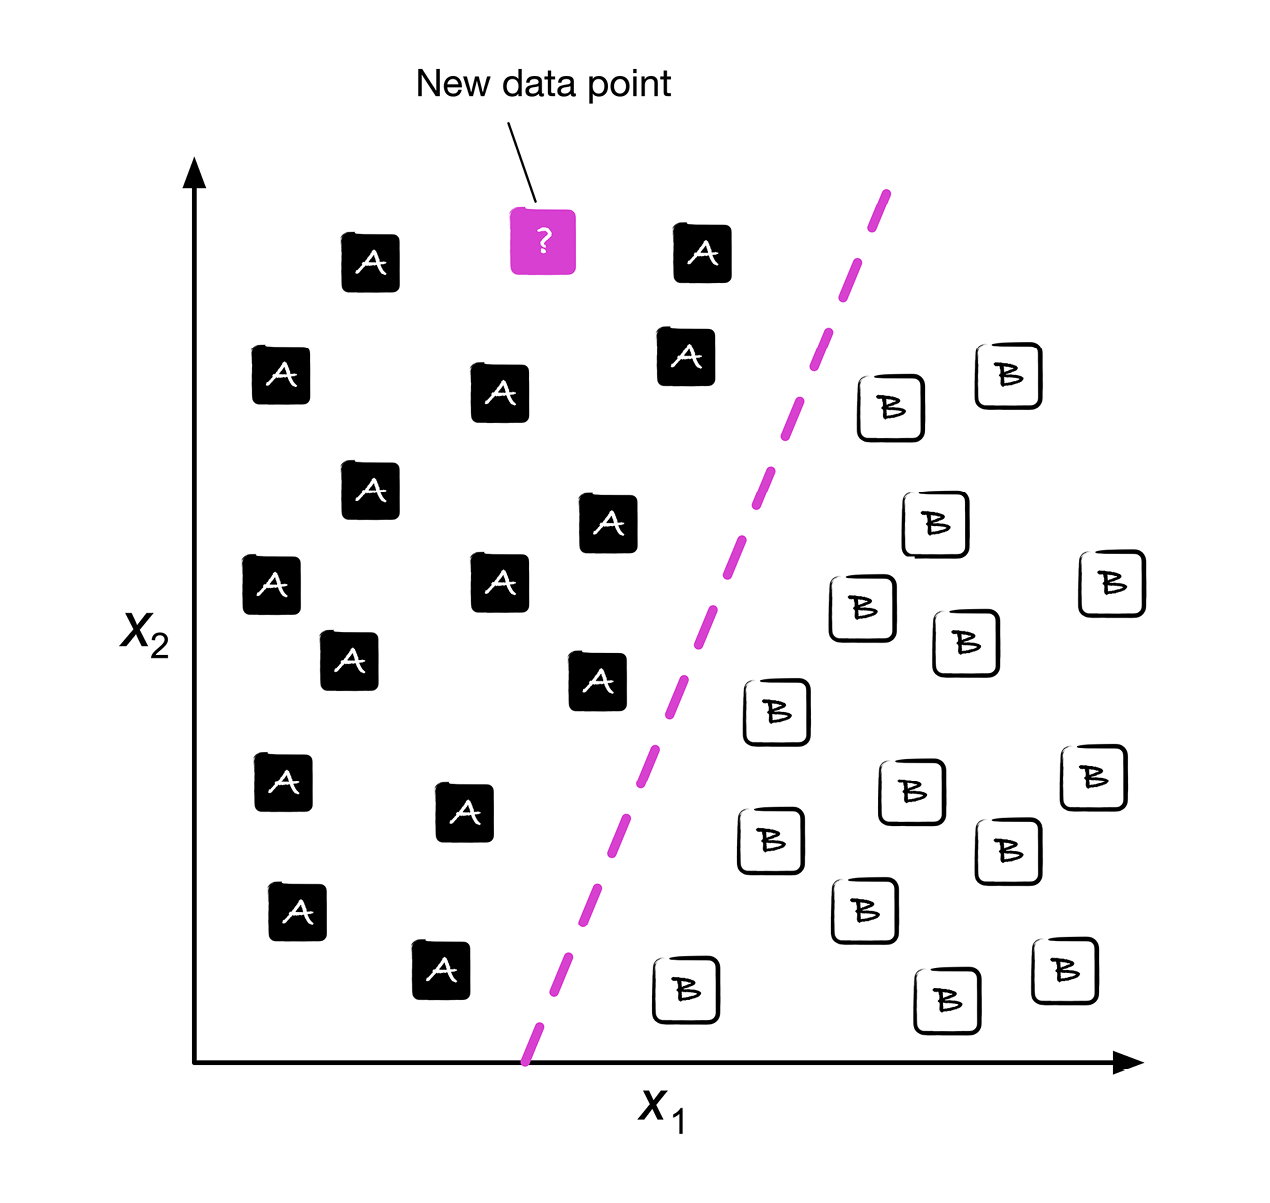
\includegraphics[scale=1]{images/classification_ml} \\
            \caption{Classification in Machine Learning}
            \label{figure:classification_ml}
        \end{minipage}
    \end{figure}

    The next ilustration shows the concept of binary classification task given 30 training examples; 15 training are labeled as \textbf{class A} and the other 15 labeled as \textbf{class B}.

    Our dataset is two-dimensional, meaning that each example has two values associated with it: $x_1$ and $x_2$. We can use a supervised machine learning algorithm to to learn a rule (decision boundary represented as the dashed line) that can separate two classes and classify new data into each of those two categories given its $x_1$ and $x_2$ values.

    \begin{obs}[\textbf{Nature of classification of class labels}]
        When a set of class labels does not have to be of a binar ynature. The predictive model learned by a supervised learning algorithm can assign any class label that was presented in the training dataset to a new, unlabeled data point or instance.
    \end{obs}

    \begin{exa}
        An example of a multiclass classification task is handwritten character recognition.
    \end{exa}

    \subsection{Regression for Predicting Continous Outcomes}

    \begin{mydef}[\textbf{Regression Analysis}]
        In a \textbf{regression analysis}, \textit{we are given a number of predictor (\textbf{explanatory}) variables and a continus response variable (\textbf{outcome}) and we try to finde a relationship between those variables that allows us to predict an outcome}.
    \end{mydef}

    \begin{obs}[\textbf{Feature and Target Variables}]
        In the field of machine learning, the predictor variables are commonly called \textit{features}, and the response variables are referred to as \textit{target variables}.
    \end{obs}

    \begin{exa}
        Let's asume we want to predict the mat SAT scores of students. If there is a relationship between time spent studying for the test and the final scores, we could use it as training data to learn a model that uses the study time to predict the test scores of future students.
    \end{exa}

    Given a feature variable $x$ and a target variable $y$, we fit a straight line to the data points that minimizes the error in predicting $y$ from $x$.

    We can now use the intercept and slope learned from this data to predict the target variable of new data.

    \begin{figure}[h]
        \begin{minipage}{\textwidth}
            \centering
            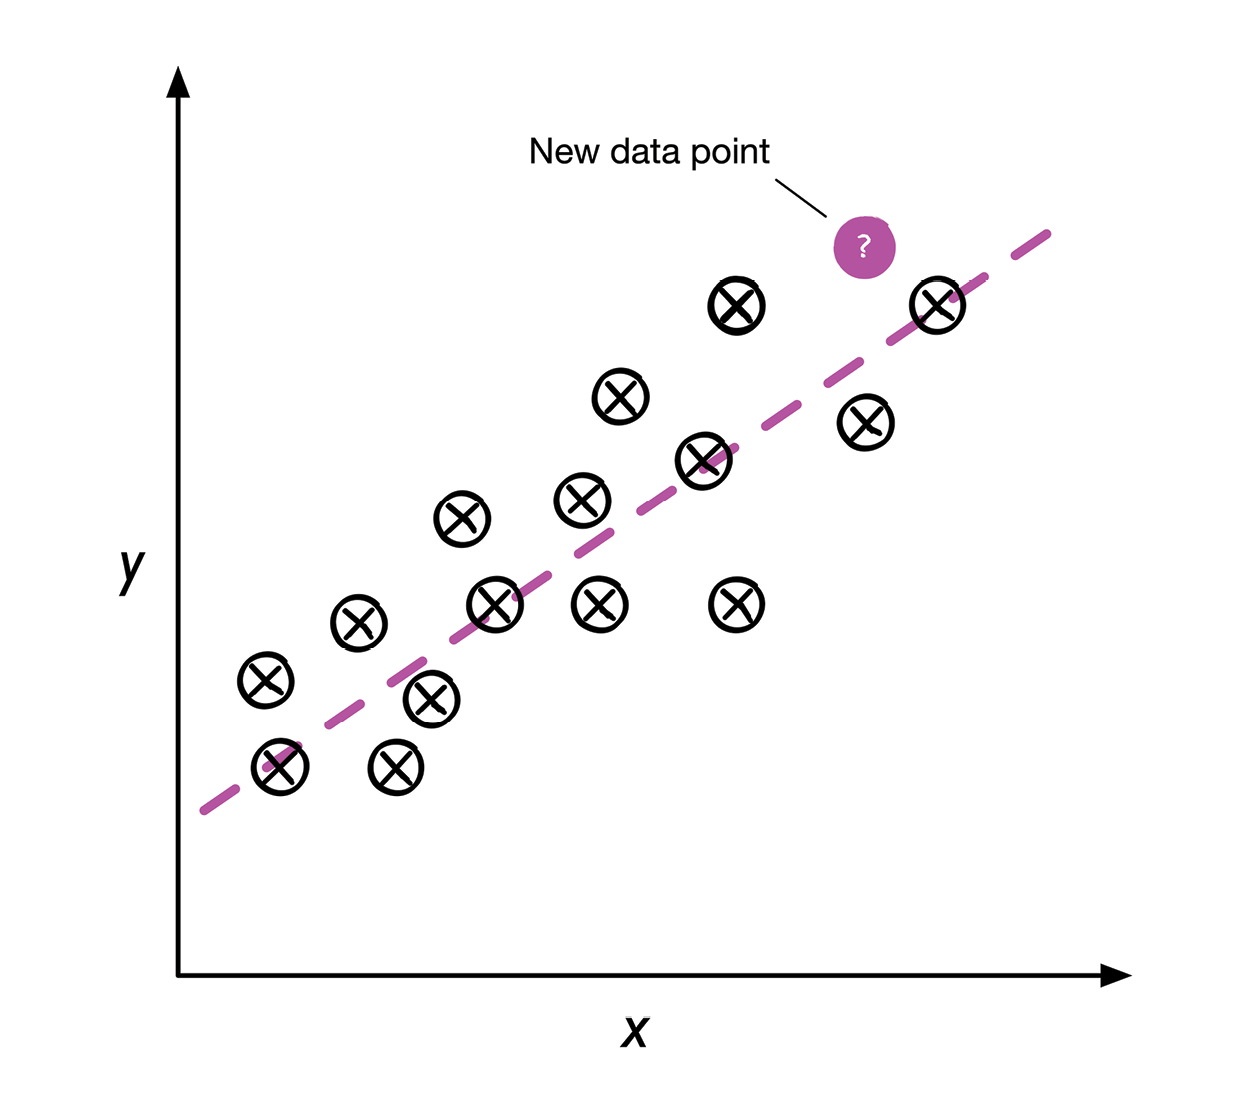
\includegraphics[scale=1]{images/linear_aproximation.png} \\
            \caption{Linear Aproximation}
            \label{figure:linear_aproximation}
        \end{minipage}
    \end{figure}

    \section{Solving Problems with Reinforcement Learning}

    \begin{mydef}[\textbf{Reinforcement Learning}]
        \textbf{Reinforcement Learning} has the \textit{goal to develop a system} (called \textbf{agent}) \textit{that improves its performance through interactions with the enviroment}.
    \end{mydef}

    \begin{obs}
        Typically, the information coming from a current state of the enviroment also includes a \textbf{reward signal}. With this in mind, reinforcement learning can be vewed as being realted to supervised learning.

        This feedback is not the correct ground-truth label or value, \textit{but a measure of how well the action is evaluated by a reward function}.
    \end{obs}

    Using a reward signal, a system can measure this reward via an exploratory trial-and-error approach or deliberative planning.

    \begin{exa}
        One of the most popular examples of reinforcement learning is \textbf{chess program}. The agent decides upon a series of moves and the reward can be defined as win or lose at the end of the game.
    \end{exa}

    In synthesis, the reinforcement learning can be described with the following diagram.

    \begin{figure}[h]
        \begin{minipage}{\textwidth}
            \centering
            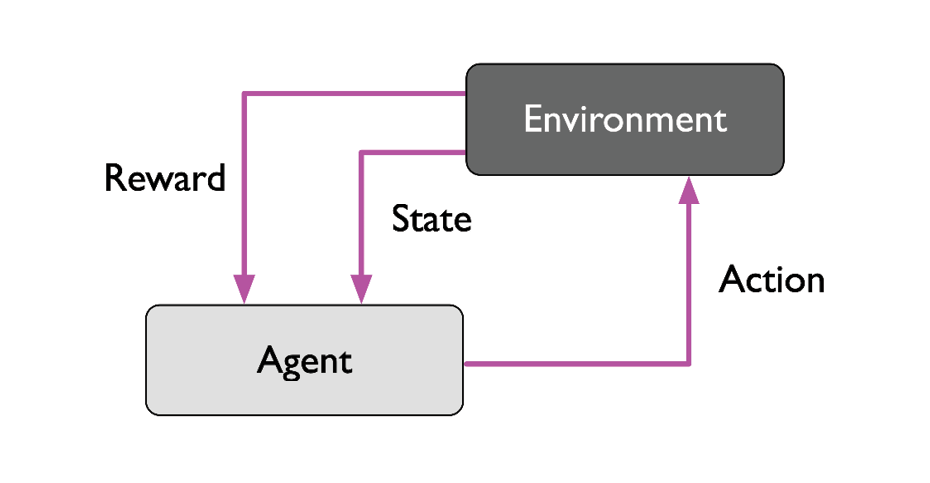
\includegraphics[scale=1]{images/_e4ebbd4.png} \\
            \caption{Reinforcement Learning Process}
            \label{figure:reinforcement_learning_process}
        \end{minipage}
    \end{figure}

    There are many different subtypes of reinforcement learning, but in a general scheme the agent tries to maximize the reward through a series of interactions with the enviroment.
    
    \begin{idea}
        In summary, reinforcement learning is concerned with learning to choose a series of actions that maximizes the total reward which could be earned immediately after taking an action or vía \textit{delayed} feedback.
    \end{idea}

    \section{Unsupervised Learning}

    Unsupervised learning tries to find the hidden structures of our data. Using supervised learning or reinforcement learning, we have the right answer or a measure of a reward for particular actions, respectively. Unsupervised learning explores the structure of our data to extract meaningful information without the guidance of a known outcome variable.

    \subsection{Finding Subgroups With Clustering}

    \begin{mydef}[\textbf{Clustering}]
        \textbf{Clustering} \textit{is an exploratory data analysis or pattern discovery technique that organizes information into meaningful subgroups} (called \textbf{clusters}) \textit{without any prior knowledge of group memberships}.
    \end{mydef}

    Each cluster defines a group of objects that share a certain degree of similarity but are more dissimilar to objects in other clusters which is why clustering is called (sometimes) \textbf{unsupervised classification}.

    The following scatter plot shows how clustering can organizse unlabeled data into three disctinct groups or clusters.

    \begin{figure}[h]
        \begin{minipage}{\textwidth}
            \centering
            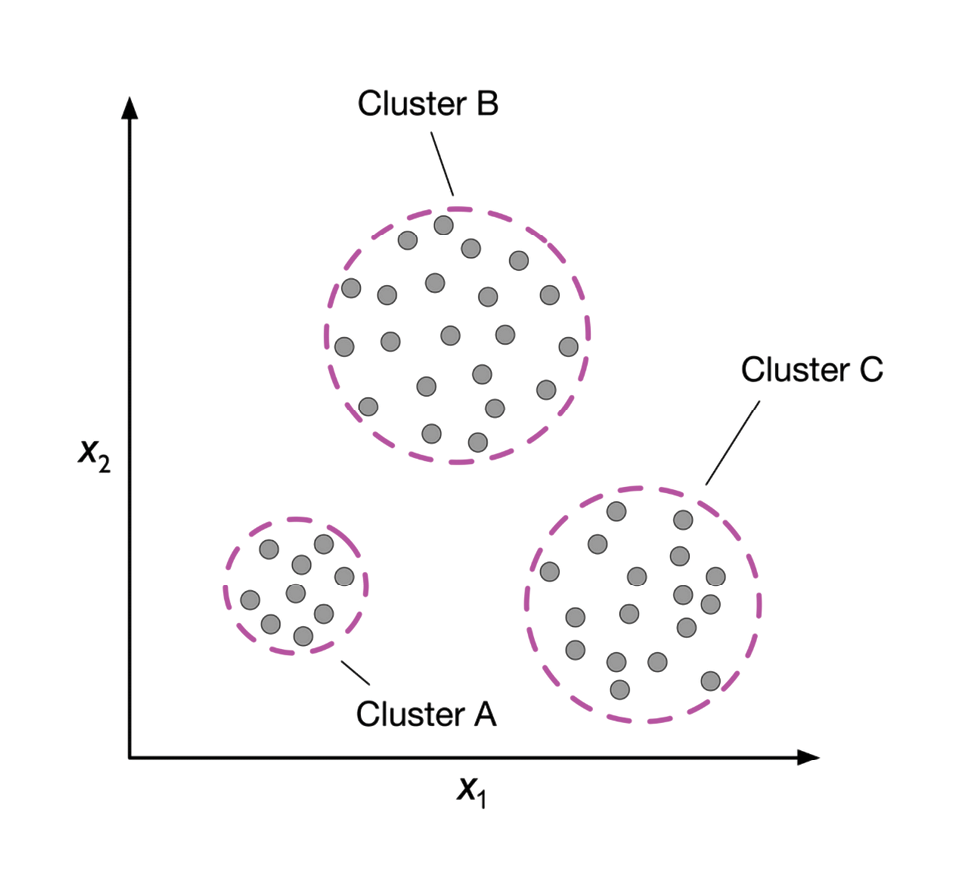
\includegraphics[scale=1]{images/_f1d6cf52eb8a474ca861d36f25bf29ef_9781801819312_01_06.png} \\
            \caption{Caption}
            \label{Texto}
        \end{minipage}
    \end{figure}

    \subsection{Dimensionality Reduction for Data Compresion}

    Another subfield of unsupervised learning is dimensionality reduction.

    \begin{mydef}[\textbf{Dimensionality Reduction}]
        \textbf{Dimensionality reduction} is the process to reduce the dimension of the data we are working it, preserving the original and meaningful data needed to interpret it.
    \end{mydef}

    Often, we work with data of high dimensionality that can present challenges for limited storage space and the computational performance of machine learning algorithms. The unsupervised deimensionality reduction is commonly used in feature preprocessing to remove noise from data, which can degrade the predictive performance of certain algorithms.

    Dimensionality reduction compresses the data into a smaller dinensional subspace while retaining most of the relevant information.

    \begin{obs}
        Sometimes, dimensionality reduction is useful for visualizing data. The following figure is a good and useful example of it.
    \end{obs}

    \begin{figure}[h]
        \begin{minipage}{\textwidth}
            \centering
            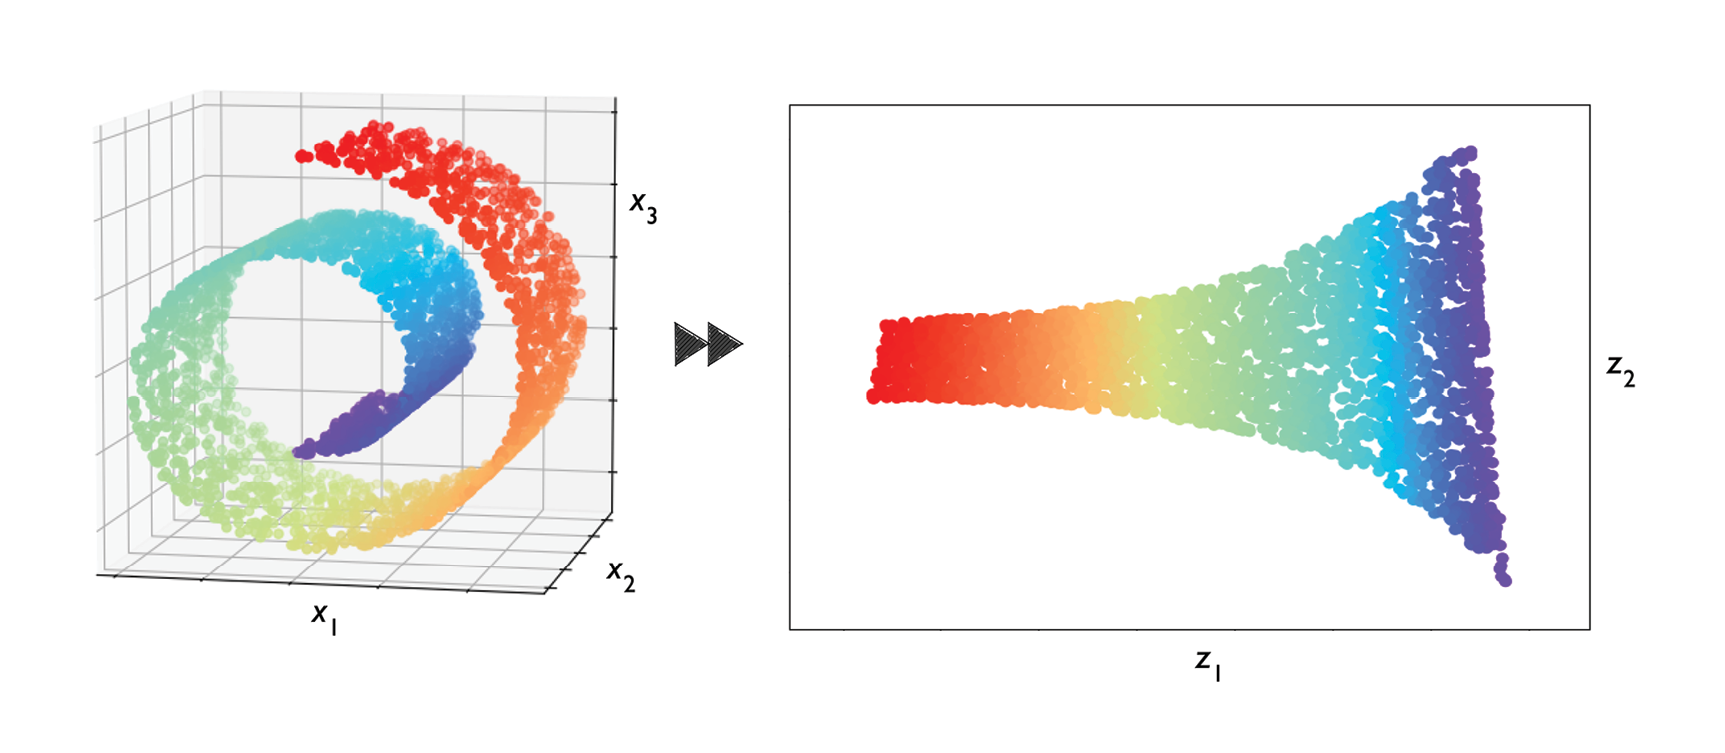
\includegraphics[scale=1]{images/_4ac24da56df8429e8ef9dfa80b7c6ea8_9781801819312_01_07.png} \\
            \caption{Example of Dimensionality Reduction in a Dataset.}
            \label{figure:dimensionality_reduction_example}
        \end{minipage}
    \end{figure}

    \section{Terminology and Notations}
    
    \begin{mydef}[\textbf{Dataset}]
        A \textbf{dataset} is a \textit{collection of related sets of information that is composed of separate elements} but can be manipulated as a unit by a computer.
    \end{mydef}

    One image that contains most of the information that we'll be using throught this course is the following:

    \begin{figure}[h]
        \begin{minipage}{\textwidth}
            \centering
            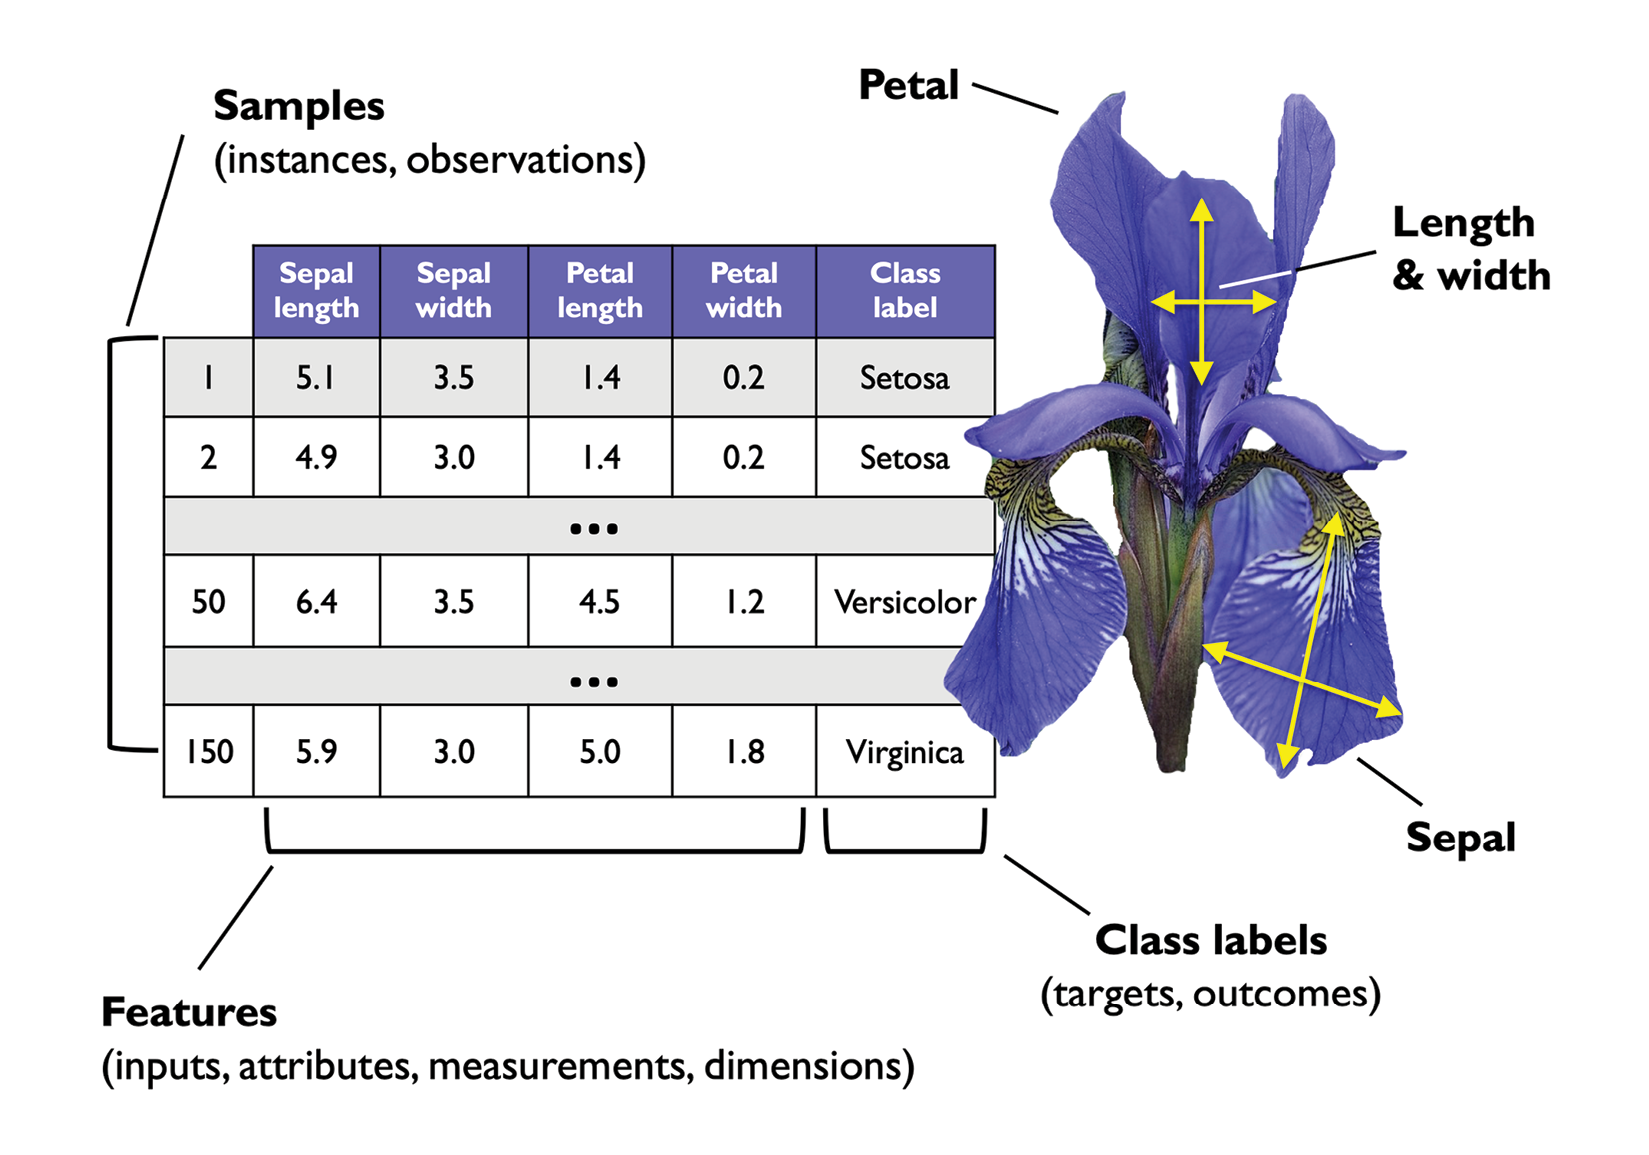
\includegraphics[scale=1]{images/definitions.png} \\
            \caption{Samples, Features, and Class labels.}
            \label{figure:samples_features_class_labels}
        \end{minipage}
    \end{figure}

    \begin{exa}
        The Iris dataset contains the measurements of 150 iris flowers from three different species (setosa, versicolor and virginica).
    \end{exa}
    
    Each flower example represents one row in our dataset and the flower measurements in centimeters are stored as columns, called \textbf{features of the dataset}.

    \begin{mydef}[\textbf{Feature}]
        In a dataset, a \textbf{feature} \textit{is an input, attribute, measurement or dimensions of something}.
    \end{mydef}

    \begin{idea}[\textbf{Notation}]
        The iris dataset consists of 150 examples and four features, we will write them as a $150\times 4$ matrix:
        \begin{equation*}
            X=\left[
                \begin{array}{c c c c}
                    x_1^{(1)} & x_2^{(1)} & x_3^{(1)} & x_4^{(1)} \\
                    x_1^{(2)} & x_2^{(2)} & x_3^{(2)} & x_4^{(2)} \\
                    \vdots & \vdots & \vdots & \vdots \\
                    x_1^{(150)} & x_2^{(150)} & x_3^{(150)} & x_4^{(150)} \\
                \end{array}
            \right]
        \end{equation*}
        Vectors will be identified as the column matrix $\vec{x}\in\bbm{R}^{n\times1}$. To refer to the elements of the matrix we will use the notation $x_i^{(j)}$.
    \end{idea}

    \begin{obs}[\textbf{Use of Notation}]
        In the latter idea, $x_1^{(150)}$ refers to the first dimension flower example 150, corresponding to the sepal length.

        Each row in the matrix $X$ represents one flower instance and can be written as a four-dimensional row vector:
        \begin{equation*}
            x^{(i)}=\left[\begin{array}{c c c c}
                x_1^{(i)} & x_2^{(i)} & x_3^{(i)} & x_4^{(i)} \\
            \end{array} \right]
        \end{equation*}

        Each feature is a 150-dimensional column vector, denoted by $x_j$:
        \begin{equation*}
            x_j=\left[ 
                \begin{array}{c}
                    x_j^{(1)} \\
                    x_j^{(2)} \\
                    \vdots \\
                    x_j^{(150)} \\
                \end{array}
            \right]
        \end{equation*}
    \end{obs}
    
    We represent the target variables (here, class labels) as 150-dimensional column vector:
    \begin{equation*}
        y=\left[ 
            \begin{array}{c}
                y^{(1)} \\
                y^{(2)} \\
                \vdots \\
                y^{(150)} \\
            \end{array}
        \right]
    \end{equation*}
    where $y^{(i)}\in\left\{\textup{Setosa},\textup{Versicolor},\textup{Virginica}\right\}$.

    \subsection{Machine Learning Teminology}

    \begin{mydef}[\textbf{Terminology in Machine Learning}]
        Some of the following terms are largely used in machine learning:
        \begin{itemize}
            \item \textbf{Training example}: A row in a table representing the dataset and synonymous with an observation, record, instance, or sample (in most contexts, sample refers to a collection of training examples).

            \item \textbf{Training}: Model fitting, for parametric models similar to parameter estimation.

            \item \textbf{Feature} ($x$): A column in a data table or data (design) matrix. Synonymous with predictor, variable, input, attribute, or covariate.

            \item \textbf{Target} ($y$): Synonymous with outcome, output, response variable, dependent variable, (class) label, and ground truth.

            \item \textbf{Loss function}: Often used synonymously with a cost function. Sometimes the loss function is also called an error function. In some literature, the term 'loss' refers to the loss measured for a single data point, and the cost is a measurement that computes the loss (average or summed) over the entire dataset.
        \end{itemize}
    \end{mydef}

    \section{Machine Learning Systems}

    In this section we'll dsicuss the other important parts of a machine learning system accompaying the learning algorithm.

    \begin{figure}[h]
        \begin{minipage}{\textwidth}
            \centering
            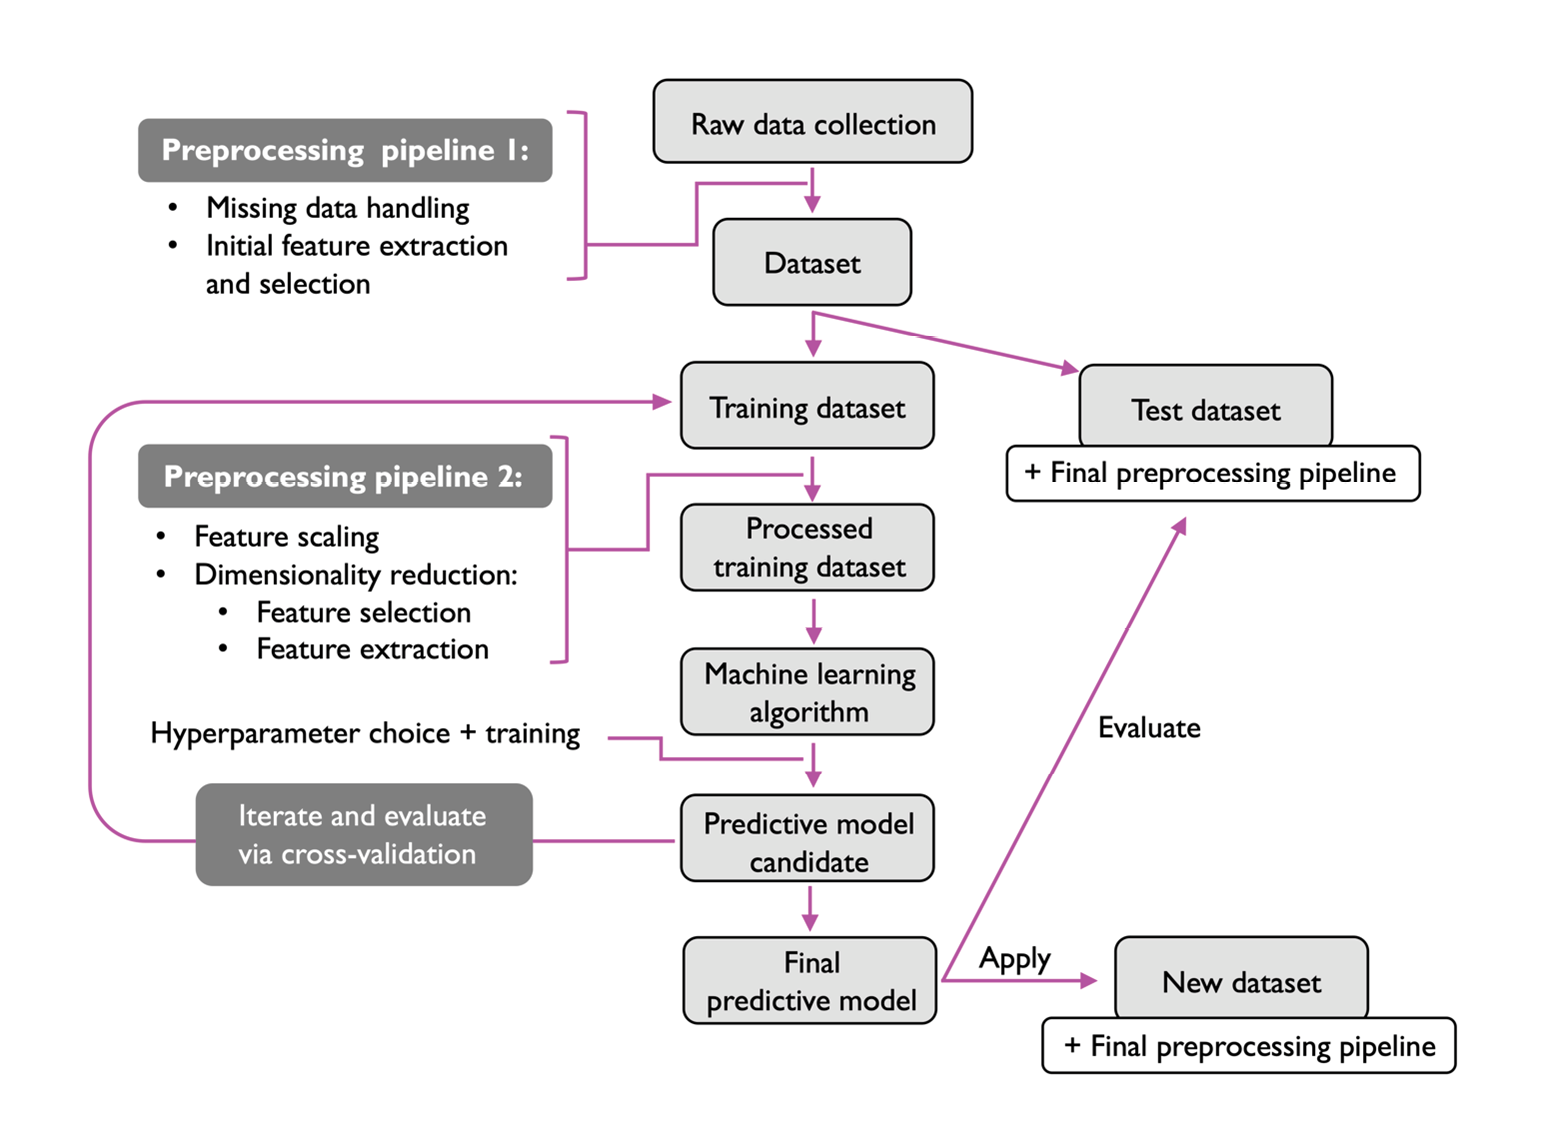
\includegraphics[scale=1]{images/machine_learning_system.png} \\
            \caption{Machine Learning System.}
            \label{figure:machine_learning_system}
        \end{minipage}
    \end{figure}

    \subsection{Preprocessing: Getting Data into Shape}

    Raw data rarely comes in the form and shape that is necessary for the optimal performance of a learning algorithm. Thus, the preprocessing of the data is one of the most crucial steps in any machine learning application.

    \begin{mydef}[\textbf{Preprocessing}]
        \textbf{Preprocessing} is the \textit{process of converting raw data into dara suitable for a machine learning algorithm}.
    \end{mydef}

    \begin{exa}[\textbf{Optimal Features in the Iris Dataset}]
        Let's consider the iris dataset from the previous example. We can think of raw data as a series of flower images from which we want to extract \textbf{meaningful features}. Useful features could be:
        \begin{itemize}
            \item Centered around the color of the flowers.
            \item Height.
            \item Length.
            \item Width.
        \end{itemize}
    \end{exa}

    \begin{obs}[\textbf{Data Convesion}]
        Many machine learning models require that the selected features are on the same scale for optimal performance, which is achieved by transforming the features to the range $[0,1]$.

        Other way to achieve this is use standard normal distribution with zero mean and unit variance.
    \end{obs}

    \begin{obs}[\textbf{Use of Dimensionaly Reduction}]
        When certain features are highly correlated and therefore, redundant, dimensionaly techniques may be useful for compressing the features onto a lower dimensional subspace.
    \end{obs}

    The main advantage of dimensionality reduction is that less storage space is required, and therefore the learning algorithm can run much faster. This can also improve the performance of a model if the dataset contains a large number of irrelevant features (or noise).

    \begin{mydef}[\textbf{Noise}]
        In data science and statistics, \textbf{noise} refers to the \textit{random, uncontrollable, and unexplained variations in the data. It is the part of the data that does not represent the underlying phenomenon you are trying to study or model}.
    \end{mydef}

    \begin{obs}[\textbf{How to Deal with Noise?}]
        You can rarely eliminate noise completely, but you can manage it.

        \begin{enumerate}[label = \textit{(\arabic*)}]
            \item \textbf{Data Cleaning \& Preprocessing}: This is the first line of defense.
            
            \begin{itemize}
                \item \textbf{Smoothing}: Applying algorithms to average out random fluctuations in time-series or signal data.
                
                \item \textbf{Binning}: Grouping numerical values into bins to smooth out small irregularities.
                
                \item \textbf{Correcting Typos}: Standardizing text entries.
            \end{itemize}
            
            \item \textbf{Collecting More Data}: A larger dataset can sometimes "drown out" the noise, as the true signal becomes stronger with more examples.
            
            \item \textbf{Using Robust Algorithms}: Some machine learning models (like Random Forests) are inherently more resistant to noise than others (like Decision Trees).
            
            \item \textbf{Feature Selection}: Removing irrelevant or redundant features that mostly contain noise.
        \end{enumerate}
    \end{obs}

    \begin{idea}
        To determine whether our machine learning algorithm performs well not only on the training dataset but also generalizes well to new data, \textit{we also want to randomly divide the dataset into separate training and test datasets}. In this way, we can measure whether our machine learning model is performing well.
    \end{idea}

    \subsection{Training and Selecting a Predictive Model}

    \begin{center}
        \textit{We cannot get learning for free.}
    \end{center}

    \begin{obs}
        Meany different machine learning models have been developed to solve different problem tasks.
    \end{obs}

    The goal is that sometimes is easier to use a certain machine learning model for some tasks than use it for other ones.

    \begin{exa}
        Each clasification algorithm has its inherent biases, and no single calssification model enjoys superiority if we do not make any assumptions about the task.
    \end{exa}

    In summary, it's essencial to compare at least a handful of different learning algotrithms in order to train and select the best performing model.

    \begin{obs}
        Before deciding which models we shall use, we have to decide upon a metric to measure performance. One commonly used metric is classification accuracy, which is defined as the proportion of correctly classified instances.
    \end{obs}

    Sometimes we may have a machine learning model which was trained using a dataset for model selection, but one question arises: what if we do not use this training dataset? To adress this issue, we can use different techniques such as cross-validation.

    \begin{mydef}[\textbf{Cross-Validation}]
        \textbf{Cross-validation} \textit{we devide further a dataset into training and validation subsets in order to estimate the generalization performance of the model}.
    \end{mydef}

    \begin{obs}[\textbf{Hyperparameters}]
        We also cannot expect that the default parameters of the different learning algorithms provided by software libraries are optimal for our specific problem task. Therefore, we will make frequent use of hyperparameter optimization techniques that help us fine-tune the performance of our model in later sections.

        We can think of those hyperparameters as parameters that are not learned from the data but represent the knobs of a model that we can turn to improve its performance.
    \end{obs}

    \subsection{Evaluating Models and Predicting Unseen Data Instances}

    After selecting a model that has been fitted on the training dataset, we can use the test dataset to estimate how well it performs on unseen data to determine the \textbf{generalization error}.

    \begin{mydef}[\textbf{Generalization Error}]
        \textbf{Generalization Error} is \textit{formally the expected error of the model on a new, random instance drawn from the same underlying data distribution}.
    \end{mydef}

    \begin{obs}[\textbf{Dataset Dependancy}]
        It is important to note that the parameters for previously mentioned procedures, such as feature scaling and dimensionality reduction, \textbf{are solely obtained from the training dataset}, and the \textbf{same parameters are later reapplied to transform the test dataset as well as any new data instances—the performance measured on the test data may be overly optimistic otherwise}.
    \end{obs}

\end{document}